\chapter{Interrogazione del data mart}
In questa sezione vengono definite le interrogazioni sui datamart che sono state effettuate.

Tutte le richieste fatte ai datamart vengono, di conseguenza, effettuate attraverso interroga-
zioni ad un DBMS Mysql.

\section{Visualizzazione utilizzi/distanze settimanali}
Lo scopo di questa interrogazione è di poter avere una panoramica ad alto livello
sugli utilizzi per ogni giorno della settimana; questo dato è utile ad 
Helbiz in maniera da poter predisporre più o meno veicoli ai cittadini.

Questo tipo di predizione permette di identificare ad altissimo livello
in quali giorni possano essere fatte più manutenzioni (togliendo quindi i veicoli dalla strada)
e in quali non ci si può permettere questo lusso.
\begin{figure}[H]                                                                                                                                                            
\centering                                                                                                                                                                   
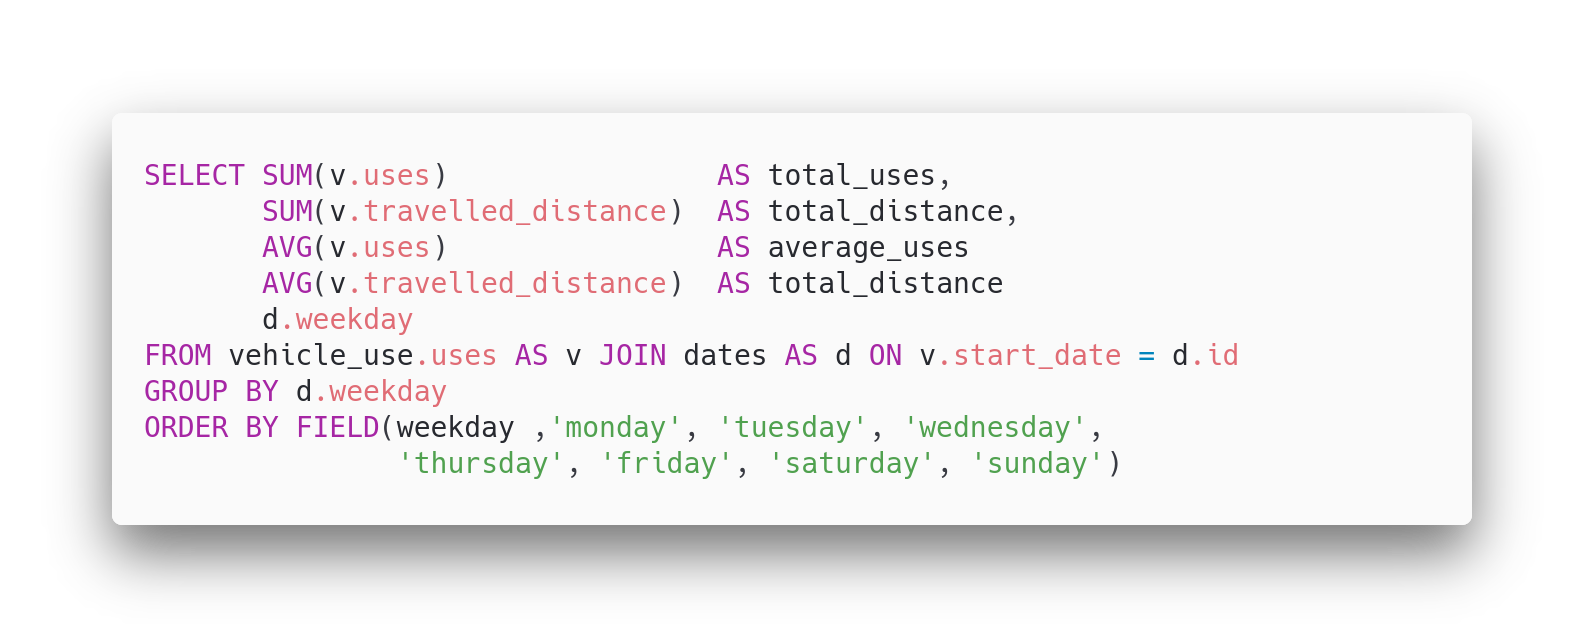
\includegraphics[width=\textwidth]{images/query1}                                                                                                                                   
\label{fig:query1}                                                                                                                                                           
\end{figure}

\iffalse
SELECT SUM(v.uses)                AS total_uses, 
	   SUM(v.travelled_distance)  AS total_distance, 
       AVG(v.uses)                AS average_uses,
       AVG(v.travelled_distance)  AS average_distance,
       d.weekday
FROM vehicle_use AS v JOIN date AS d ON v.start_time = d.id
GROUP BY d.weekday
ORDER BY FIELD(weekday ,'monday', 'tuesday', 'wednesday',
			   'thursday', 'friday', 'saturday', 'sunday')
\fi

\begin{table}[H]
\centering
\resizebox{\textwidth}{!}{%
\begin{tabular}{|
>{\columncolor[HTML]{FFFFFF}}c |c|c|c|c|}
\hline
\cellcolor[HTML]{3166FF}{\color[HTML]{FFFFFF} \textbf{Giorno}} & \cellcolor[HTML]{3166FF}{\color[HTML]{FFFFFF} \textbf{Totale Utilizzi}} & \cellcolor[HTML]{3166FF}{\color[HTML]{FFFFFF} \textbf{Totale Distanza (Km)}} & \cellcolor[HTML]{3166FF}{\color[HTML]{FFFFFF} \textbf{Media Utilizzi}} & \cellcolor[HTML]{3166FF}{\color[HTML]{FFFFFF} \textbf{Media Distanza (Km)}} \\ \hline
{\color[HTML]{000000} Lunedì}                                  & \cellcolor[HTML]{FF9494}1410                                            & \cellcolor[HTML]{FF8686}907                                                  & \cellcolor[HTML]{FF5555}15                                             & \cellcolor[HTML]{FF6666}9                                                   \\ \hline
{\color[HTML]{000000} Martedì}                                 & \cellcolor[HTML]{FF4040}1714                                            & \cellcolor[HTML]{FF5151}1013                 & \cellcolor[HTML]{FF7F7F}14                                             & \cellcolor[HTML]{FF3333}10                                                  \\ \hline
{\color[HTML]{000000} Mercoledì}                               & \cellcolor[HTML]{FFC8C8}1229                                            & \cellcolor[HTML]{FFB2B2}818                                                  & \cellcolor[HTML]{FFAAAA}13                                             & \cellcolor[HTML]{FF6666}9                                                   \\ \hline
{\color[HTML]{000000} Giovedì}                                 & \cellcolor[HTML]{FFBABA}1279                                            & \cellcolor[HTML]{FFC9C9}771                                                  & \cellcolor[HTML]{FFEFEF}11                                             & \cellcolor[HTML]{FFEFEF}6                                                   \\ \hline
{\color[HTML]{000000} Venerdì}                                 & \cellcolor[HTML]{FF0000}{\color[HTML]{FFFFFF} \textbf{1935}}            & \cellcolor[HTML]{FF0000}{\color[HTML]{FFFFFF} \textbf{1177}}                                                 & \cellcolor[HTML]{FF2A2A}16                                             & \cellcolor[HTML]{FF9999}8                                                   \\ \hline
{\color[HTML]{000000} Sabato}                                  & \cellcolor[HTML]{FFEFEF}1036                                            & \cellcolor[HTML]{FFEFEF}664                                                  & \cellcolor[HTML]{FF7F7F}14                                             & \cellcolor[HTML]{FF6666}9                                                   \\ \hline
{\color[HTML]{000000} Domenica}                                & \cellcolor[HTML]{FF5B5B}1612                                            & \cellcolor[HTML]{FF3838}1060                                                 & \cellcolor[HTML]{FF0000}{\color[HTML]{FFFFFF} \textbf{17}}             & \cellcolor[HTML]{FF0000}{\color[HTML]{FFFFFF} \textbf{11}}                  \\ \hline
\end{tabular}%
}
\end{table}

Si può notare come la domenica ci siano utilizzi più frequenti ma con bassa percorrenza: questo dato potrebbe essere collegato al turismo che di solito è più frequente durante il weekend.

Nelle giornate lavorative si ha un graduale discesa dell'utilizzo per poi avere un picco di venerdì: è normale avere spostamenti di questo genere in quanto il venerdì dichiara la fine
della settimana lavorativa e vi è più voglia da parte della gente di frequentare i locali della città .

\begin{figure}[H]                                                                                                                                                            
\centering                                                                                                                                                                   
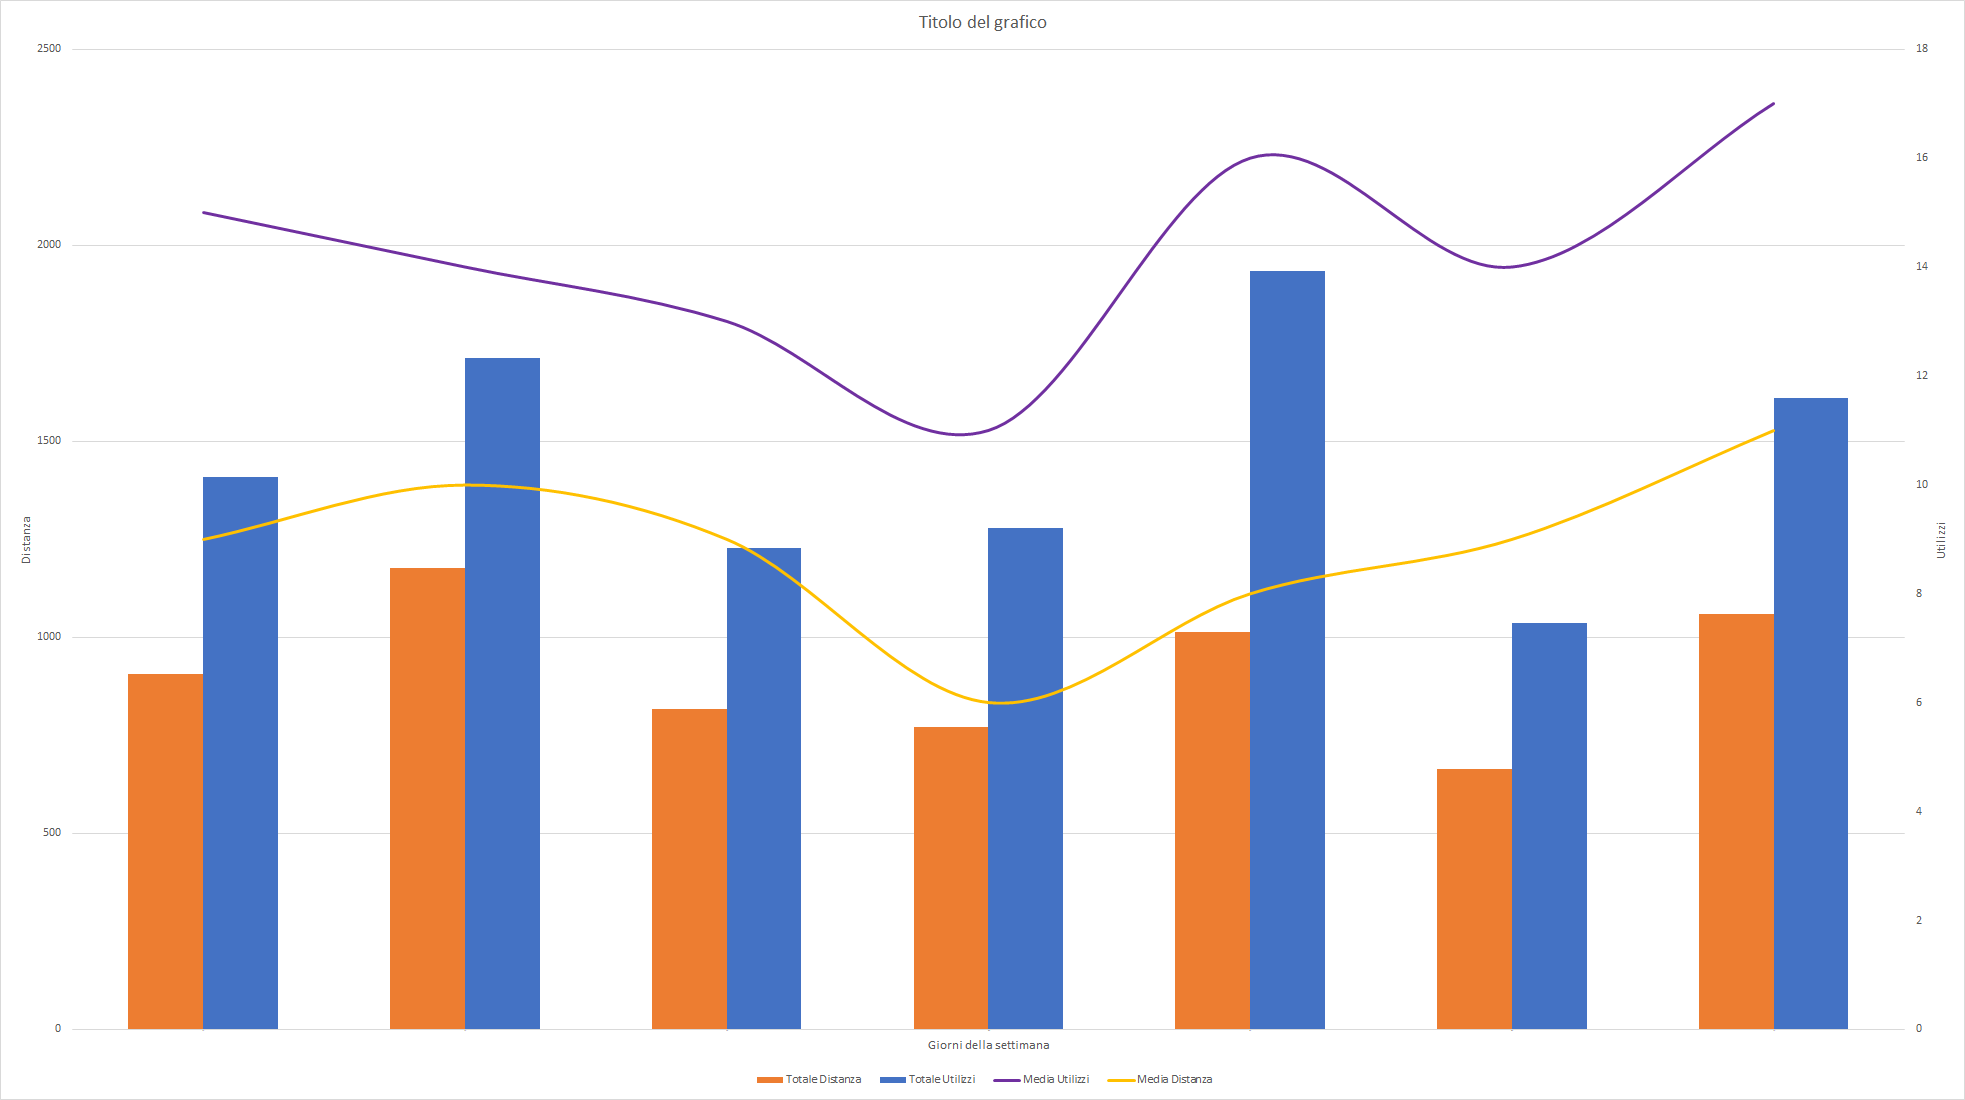
\includegraphics[width=\textwidth]{images/result12}                                                                                                                                   
\label{fig:result12}                                                                                                                                                           
\end{figure}


\section{Utilizzo per livelli di pioggia mese per mese}
La pioggia è uno dei maggiori deterrenti per impedire alle persone di
utilizzare i veicoli come monopattini o biciclette.

È quindi molto interessante capire a seconda della stagione quale
sia il livello di "sopportazione della pioggia" dell'utenza; come prima,
l'obiettivo è quello di capire in quali circostanze è possibile ritirare
più veicoli dalle strade o se adirittura decidere di sospendere il servizio: in
certe circostanze può essere un costo senza guadagno mantenere attivo l'apparato
di Helbiz se l'utenza è nulla per lunghi periodi di tempo.
Questo significa che grazie a questi dati, se in un determinato periodo futuro
dell'anno si dovessero presentare N giorni di pioggia con un livello maggiore ad M,
allora è conveniente sospendere il servizio.
\begin{figure}[H]                                                                                                                                                            
\centering                                                                                                                                                                   
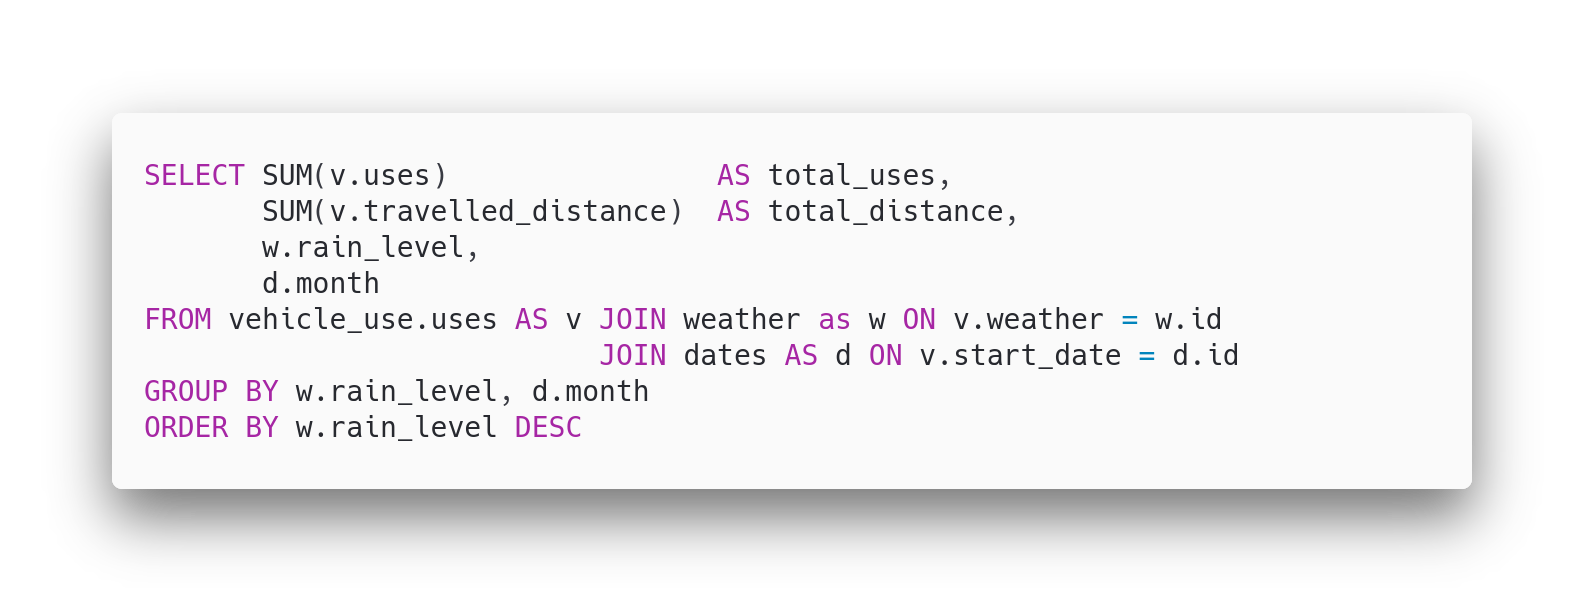
\includegraphics[width=\textwidth]{images/query2}                                                                                                                                   
\label{fig:query2}                                                                                                                                                           
\end{figure}
\iffalse
SELECT SUM(v.uses)                AS total_uses, 
	   SUM(v.travelled_distance)  AS total_distance,
       w.rain_level,
       d.month
FROM vehicle_use AS v JOIN weather as w ON v.weather = w.id
					  JOIN date AS d ON v.start_time = d.id
GROUP BY w.rain_level, d.month
ORDER BY w.rain_level DESC
\fi





\section{Confronto degli utilizzi durante uno sciopero per fascia oraria per tipo di veicolo}
Forse uno dei dati più importanti non solo Helbiz ma anche per il comune e 
i cittadini stessi; grazie a queste informazioni Helbiz può gestire durante 
un periodo critico come quello di sciopero il numero di mezzi da mettere a disposizione,
pianificando per ogni ora la strategia migliore per l'immissione di ulteriori veicoli.
\begin{figure}[H]                                                                                                                                                            
\centering                                                                                                                                                                   
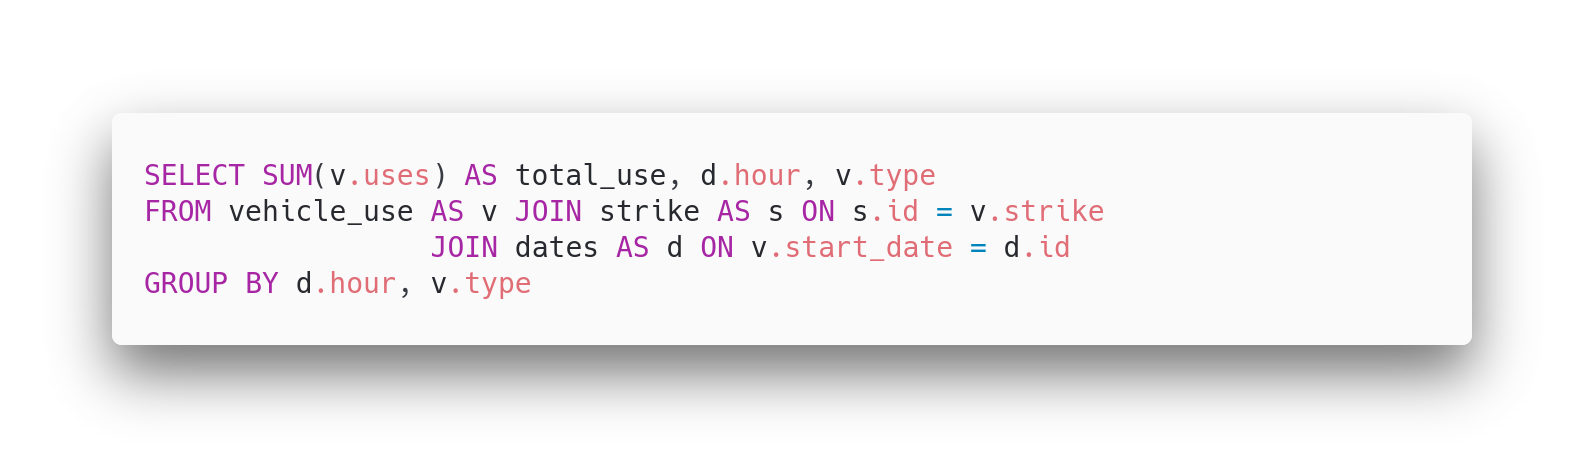
\includegraphics[width=\textwidth]{images/query3}                                                                                                                                   
\label{fig:query3}                                                                                                                                                           
\end{figure}
\iffalse
SELECT SUM(v.uses) AS total_use, d.hour, v.type
FROM vehicle_use AS v JOIN strike AS s ON s.id = v.strike
				 JOIN dates AS d ON v.start_date = d.id
GROUP BY d.hour, v.type
\fi

Purtroppo ad oggi per la città di Torino non sono presenti dati relativi alle
biciclette ma esclusivamente ai monopattini.

\begin{figure}[H]                                                                                                                                                            
\centering                                                                                                                                                                   
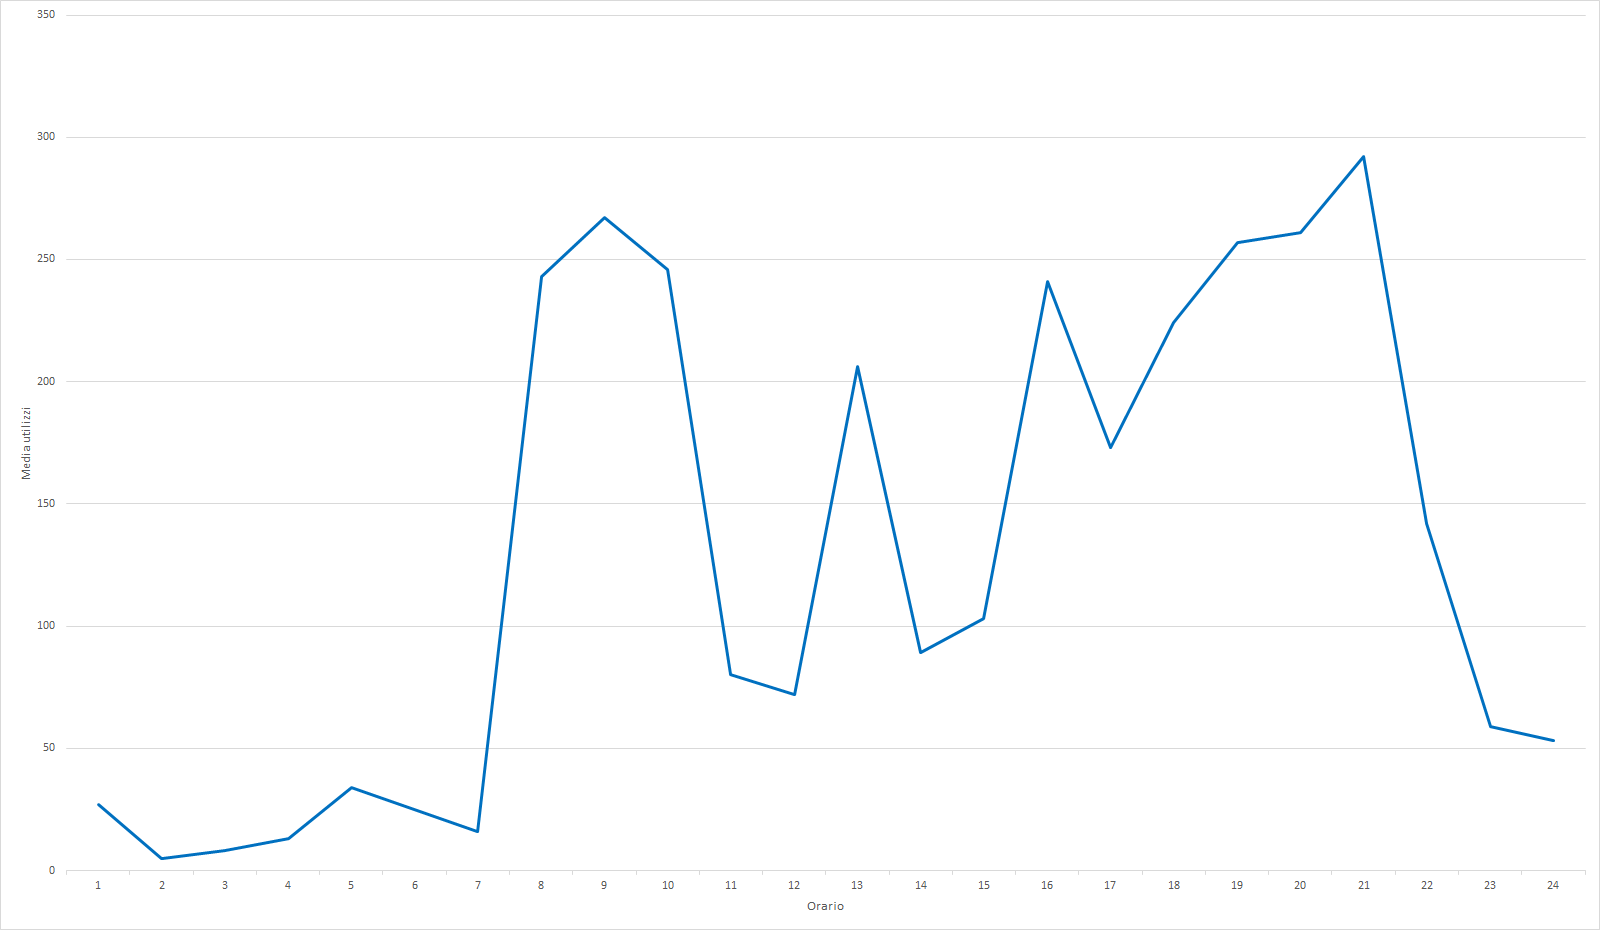
\includegraphics[width=\textwidth]{images/result3}                                                                                                                                   
\label{fig:result3}                                                                                                                                                           
\end{figure}


\section{Delta utilizzi al variare delle temperature a dipendere della presenza di scioperi}
Un altro deterrente per gli utenti è la temperatura; ma la presenza di scioperi potrebbe
far crescere il numero della domanda in quanto un utente è più predisposto a utilizzare un 
monopattino durante una giornata fredda se si trova senza possibilità di scelta.

\begin{figure}[H]                                                                                                                                                            
\centering                                                                                                                                                                   
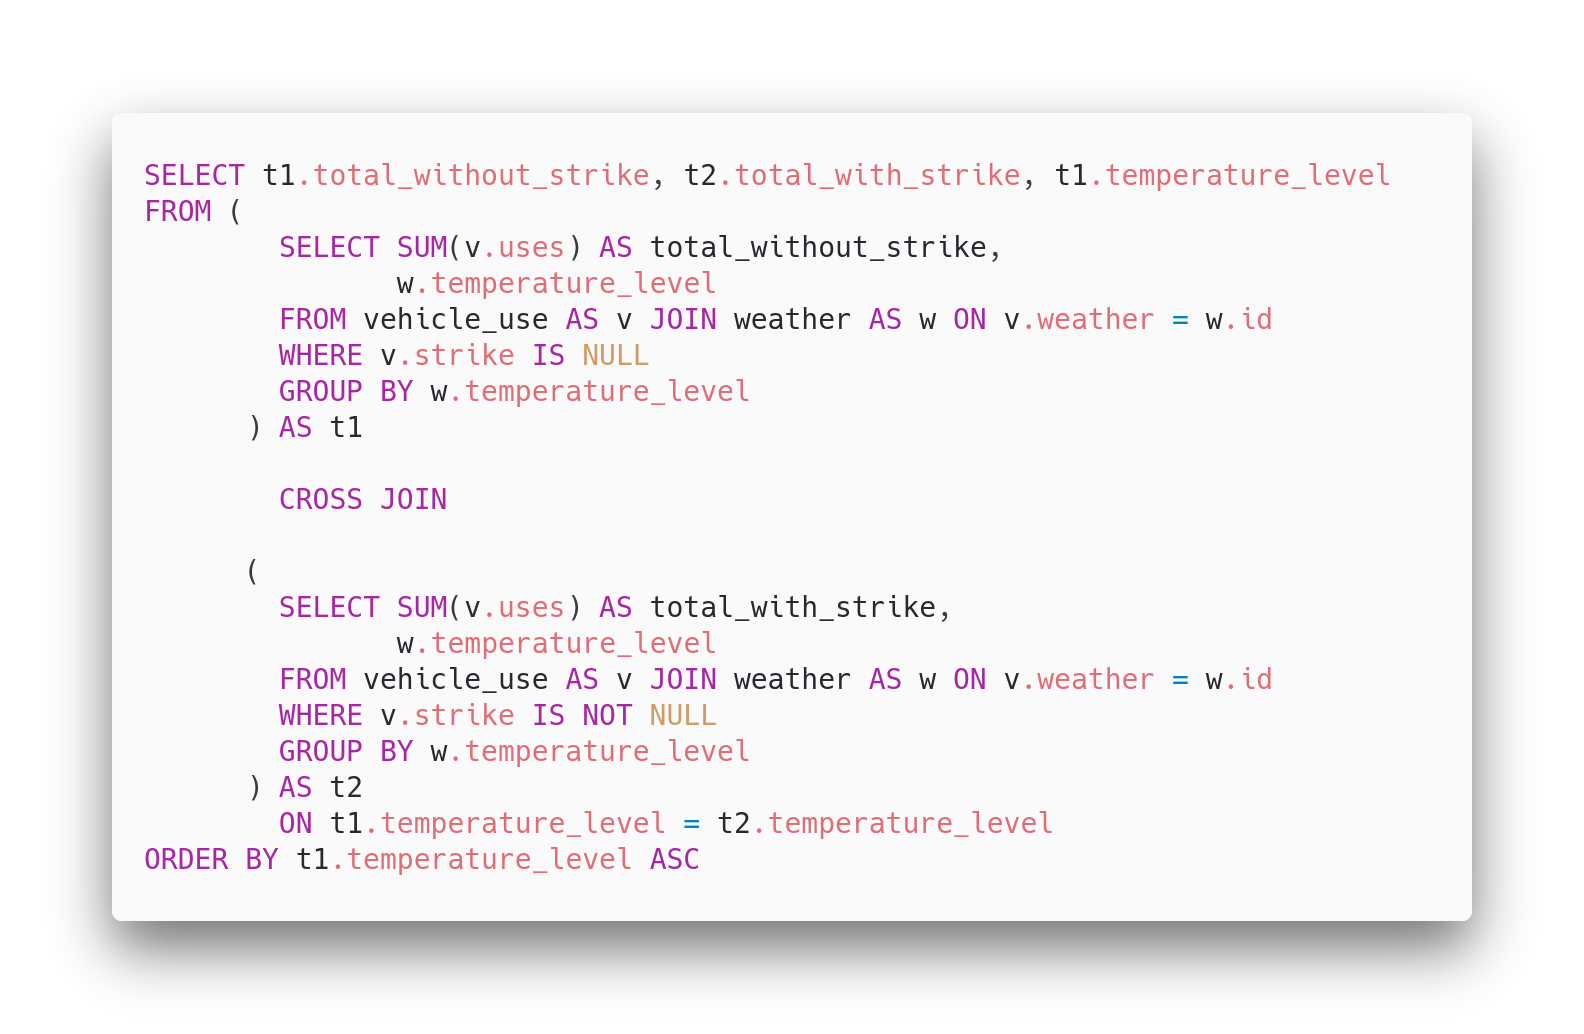
\includegraphics[width=\textwidth]{images/query4}                                                                                                                                   
\label{fig:query4}                                                                                                                                                           
\end{figure}
\iffalse
SELECT t1.total_without_strike, t2.total_with_strike, t1.temperature_level
FROM (
		SELECT SUM(v.uses) AS total_without_strike, 
  			   w.temperature_level
  		FROM vehicle_use AS v JOIN weather AS w ON v.weather = w.id
  		WHERE v.strike IS NULL
  		GROUP BY w.temperature_level
      ) AS t1 
      	
        CROSS JOIN
      
      (
        SELECT SUM(v.uses) AS total_with_strike, 
               w.temperature_level
  		FROM vehicle_use AS v JOIN weather AS w ON v.weather = w.id
        WHERE v.strike IS NOT NULL
  		GROUP BY w.temperature_level
      ) AS t2
        ON t1.temperature_level = t2.temperature_level
ORDER BY t1.temperature_level ASC
\fi

\begin{figure}[H]                                                                                                                                                            
\centering                                                                                                                                                                   
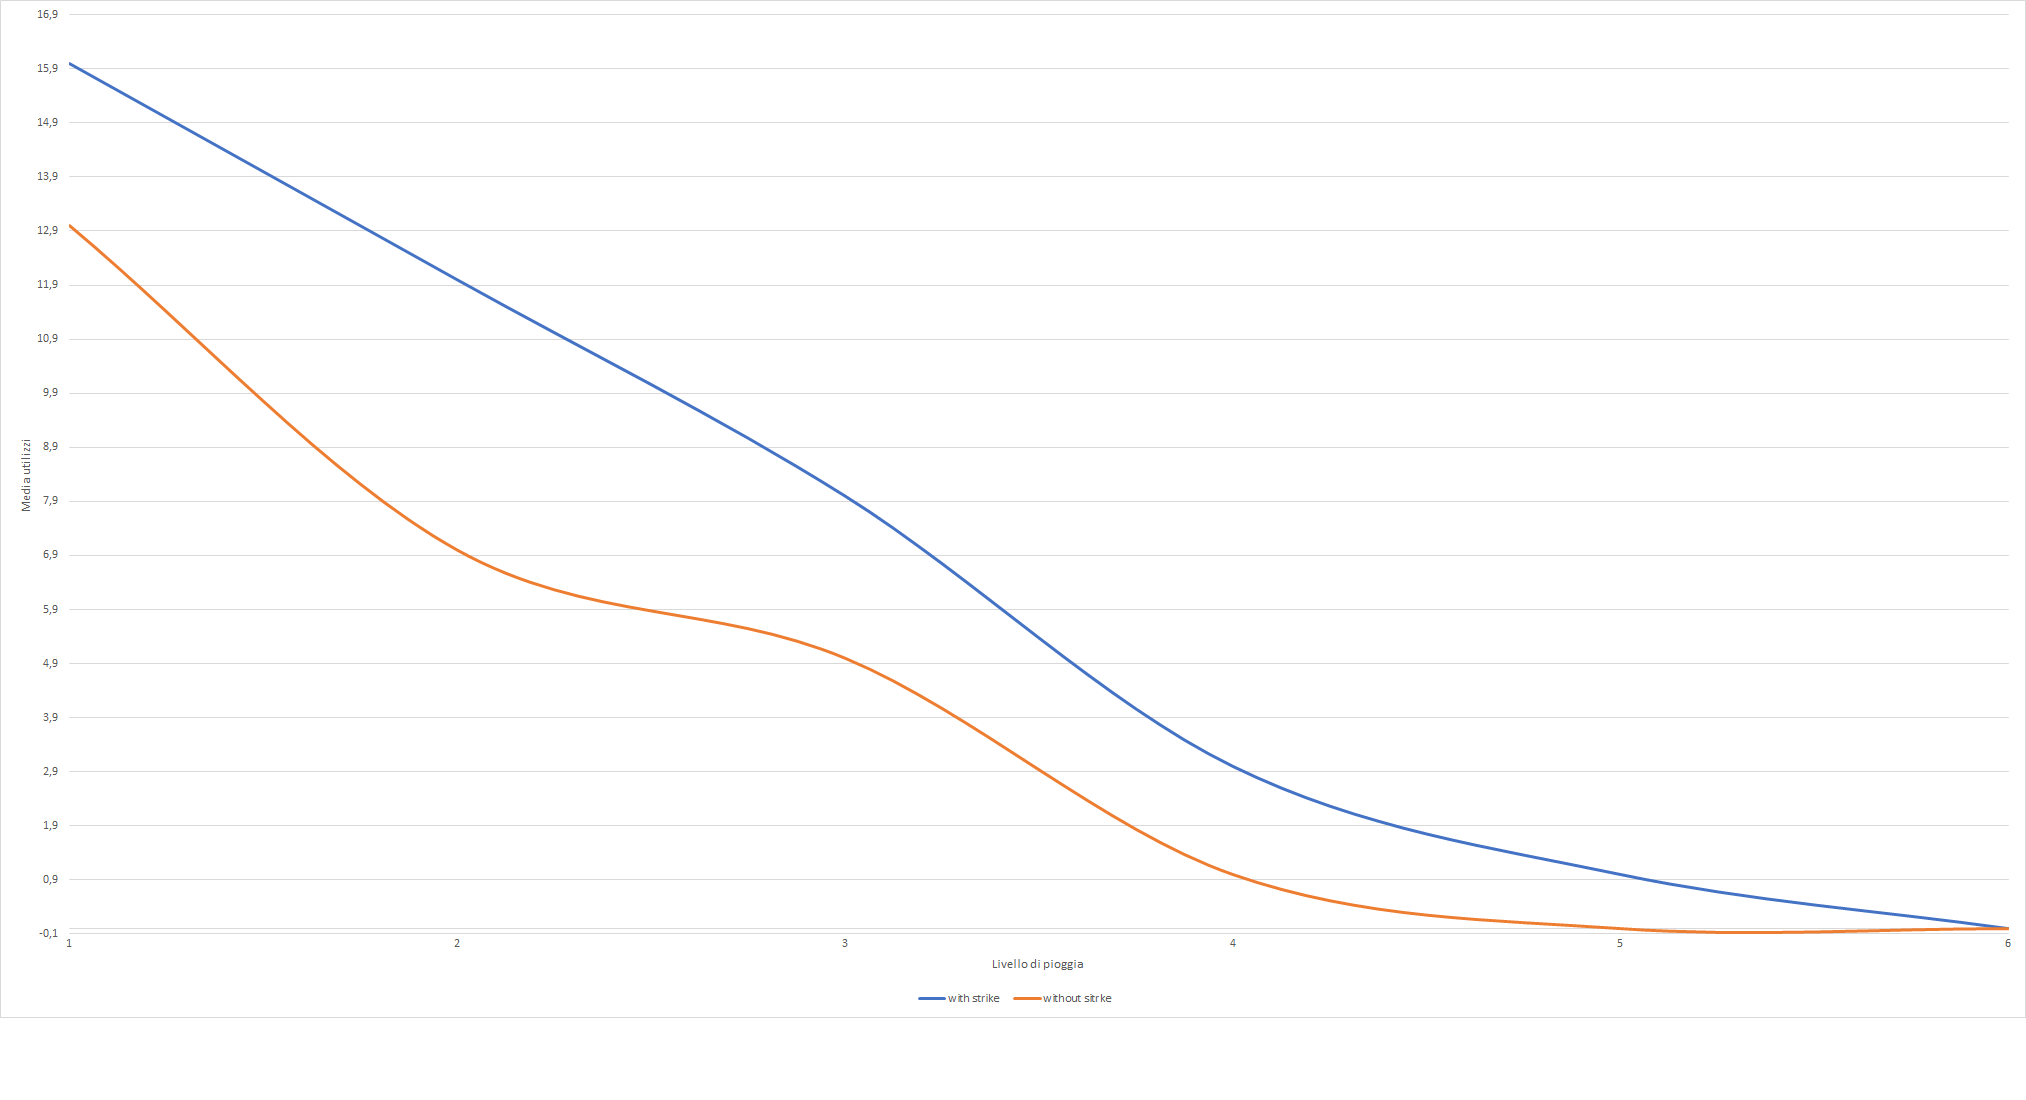
\includegraphics[width=\textwidth]{images/result4}                                                                                                                                   
\label{fig:result4}                                                                                                                                                           
\end{figure}



\section{Numero di utilizzi durante uno sciopero nelle ore di punta}
Questa interrogazione analizza ancora più nel dettaglio la situazione durante
uno sciopero e serve a capire quale sia l'effettiva domanda
da parte dell'utenza nelle fasce orarie più critiche durante uno sciopero.
Queste fasce sono quelle identificate come "orario di punta" e sono 
determinate dall'alto traffico generato dai lavoratori durante il tragitto casa-lavoro e lavoro-casa.
\begin{figure}[H]                                                                                                                                                            
\centering                                                                                                                                                                   
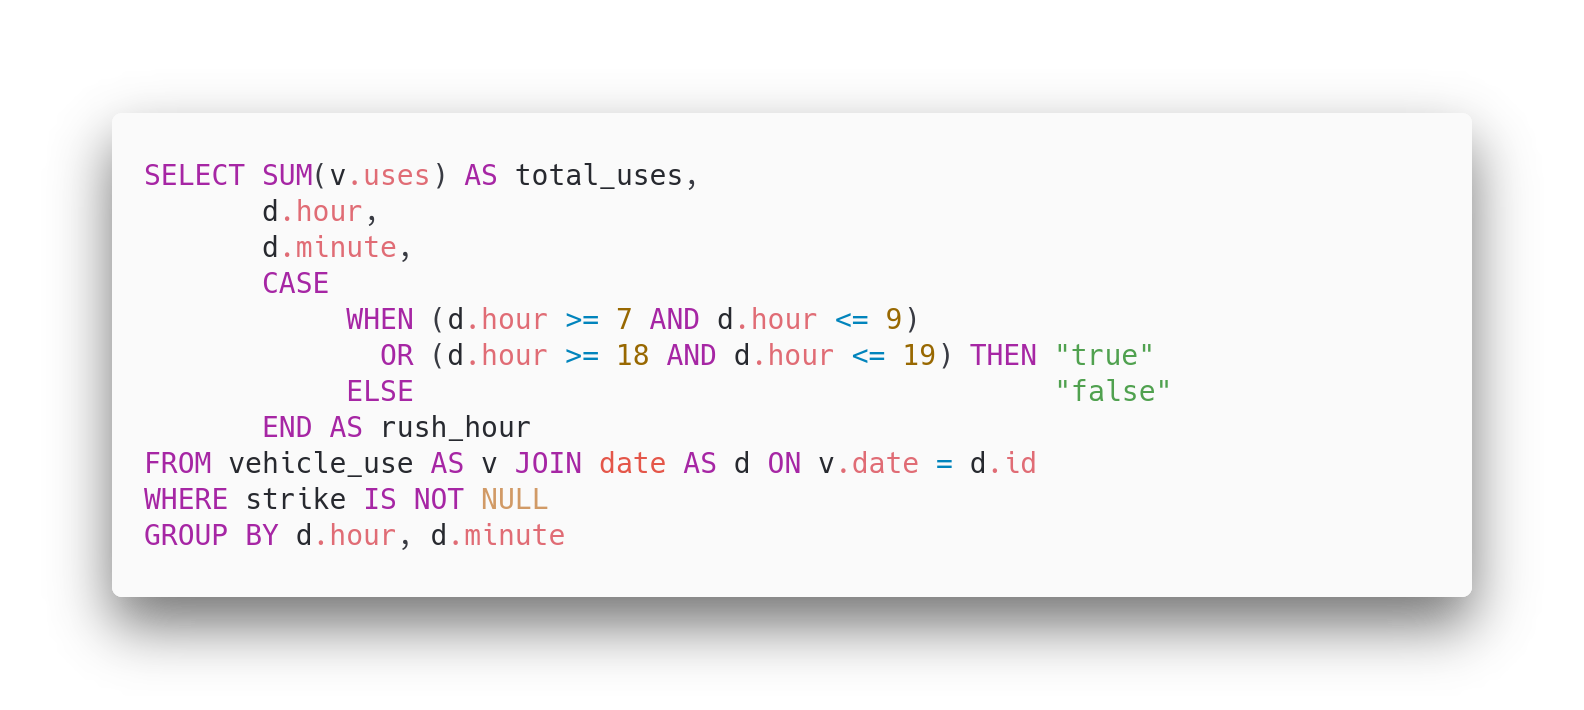
\includegraphics[width=\textwidth]{images/query5}                                                                                                                                   
\label{fig:query5}                                                                                                                                                           
\end{figure}
\iffalse
SELECT SUM(v.uses) AS total_uses, 
       d.hour,
       CASE 
       		WHEN (d.hour >= 7 AND d.hour <= 9)   
           	  OR (d.hour >= 18 AND d.hour <= 19) THEN "true"
       		ELSE 								      "false"
       END AS rush_hour
FROM vehicle_use AS v JOIN date AS d ON v.start_time = d.id
WHERE strike IS NOT NULL
GROUP BY d.hour
\fi

Si nota subito che il 41\% degli utilizzi del giorno viene fatto solo in queste 5 ore.
\begin{figure}[H]                                                                                                                                                            
\centering                                                                                                                                                                   
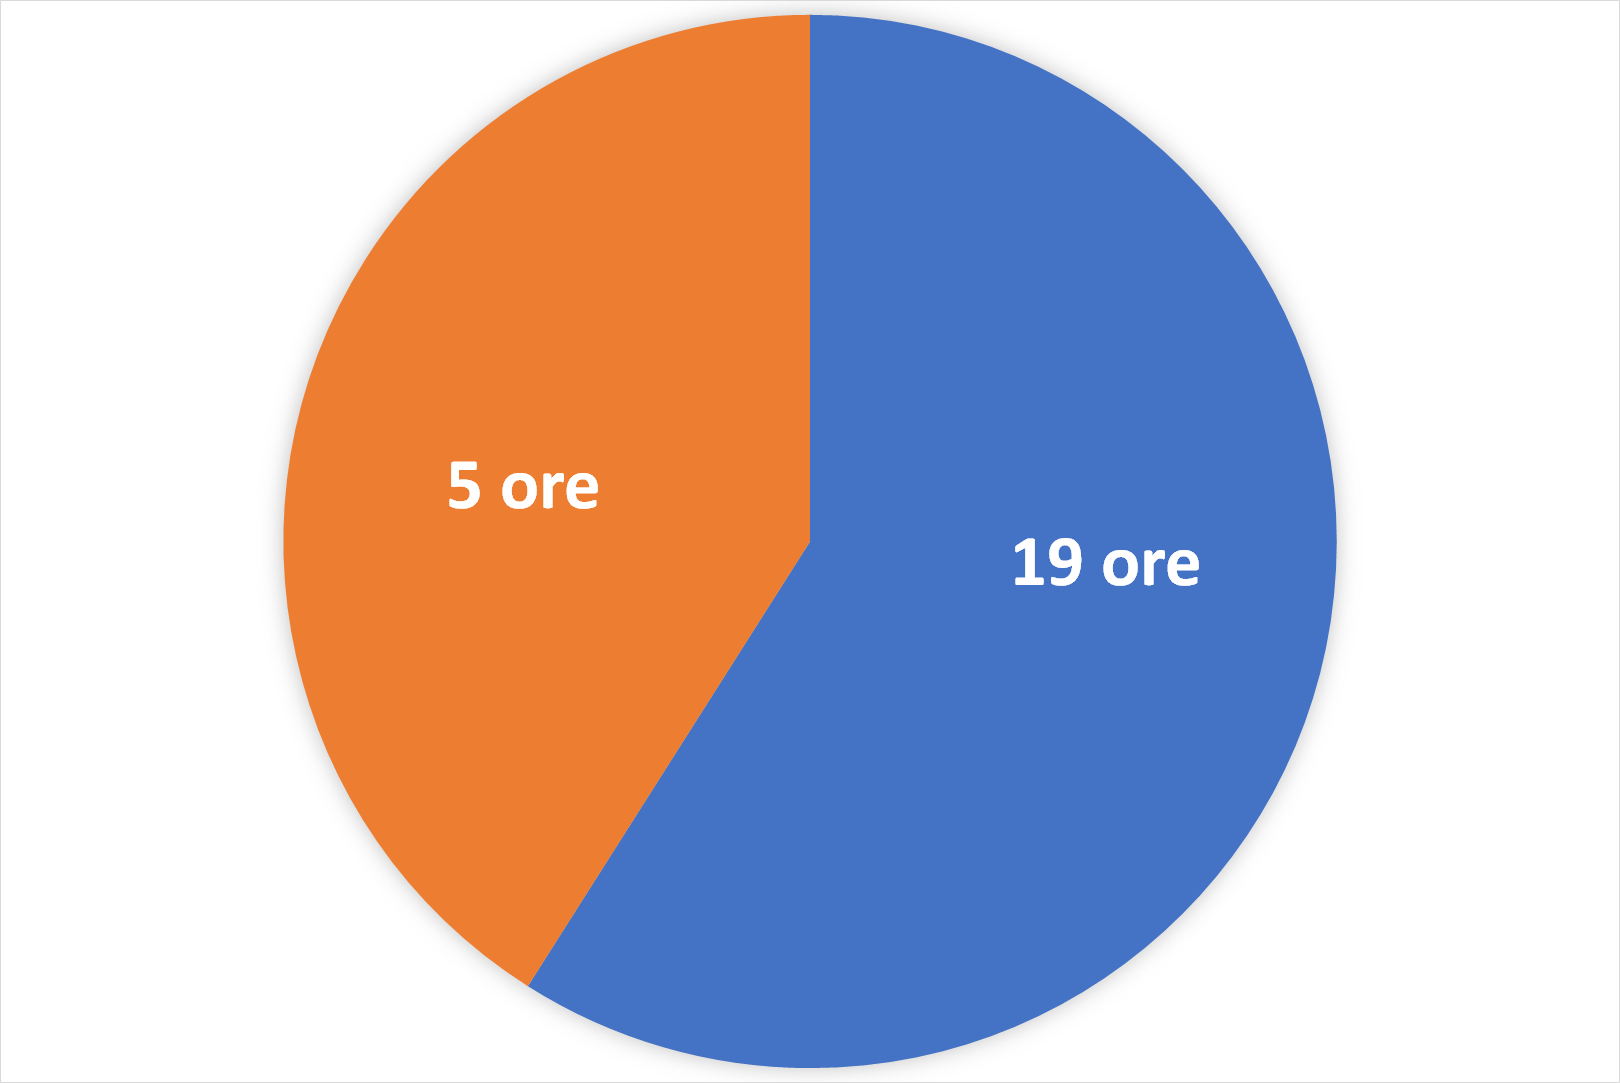
\includegraphics[width=\textwidth]{images/result5}                                                                                                                                   
\label{fig:result5}                                                                                                                                                           
\end{figure}
Risulta quindi vitale per Helbiz riuscire a gestire i due periodi che vanno dalle 7 alle 9  e dalle 18 alle 19.


\section{Numero di utilizzi durante diverse fasce orarie}
Questa interrogazione, molto simile alla precendente, invece analizza
tutte le fasce orarie indipendentemente dal fatto che ci sia o meno uno sciopero.
Le fasce orarie identificate sono
\begin{itemize}
	\item{\textbf{Orario di punta:} come spiegato nella sezione precendete, è l'orario di maggior traffico causato dai lavoratori}
	\item{\textbf{Orario lavorativo}}
	\item{\textbf{Uscita da scuola} è l'orario di uscita per la maggior parte degli studenti della scuola dell'obbligo}
	\item{\textbf{Uscita da scuola 2} simile a quella precedente, ma riguarda la fascia pomeridiana}
\end{itemize}

Queste fasce non sono solo utili a capire il numero di veicoli da mettere a disposizione, ma indicano grossolanamente quale sia 
la fascia d'età degli utilizzatori. Questa informazione diventa molto utile in fase promozionale del servizio (\emph{e.g.} se nella fascia d'orario
uscita scuole non si nota abbastanza affluenza, si potrebbe pensare di creare una agevolazione in collaborazione con le scuole).

\begin{figure}[H]                                                                                                                                                            
\centering                                                                                                                                                                   
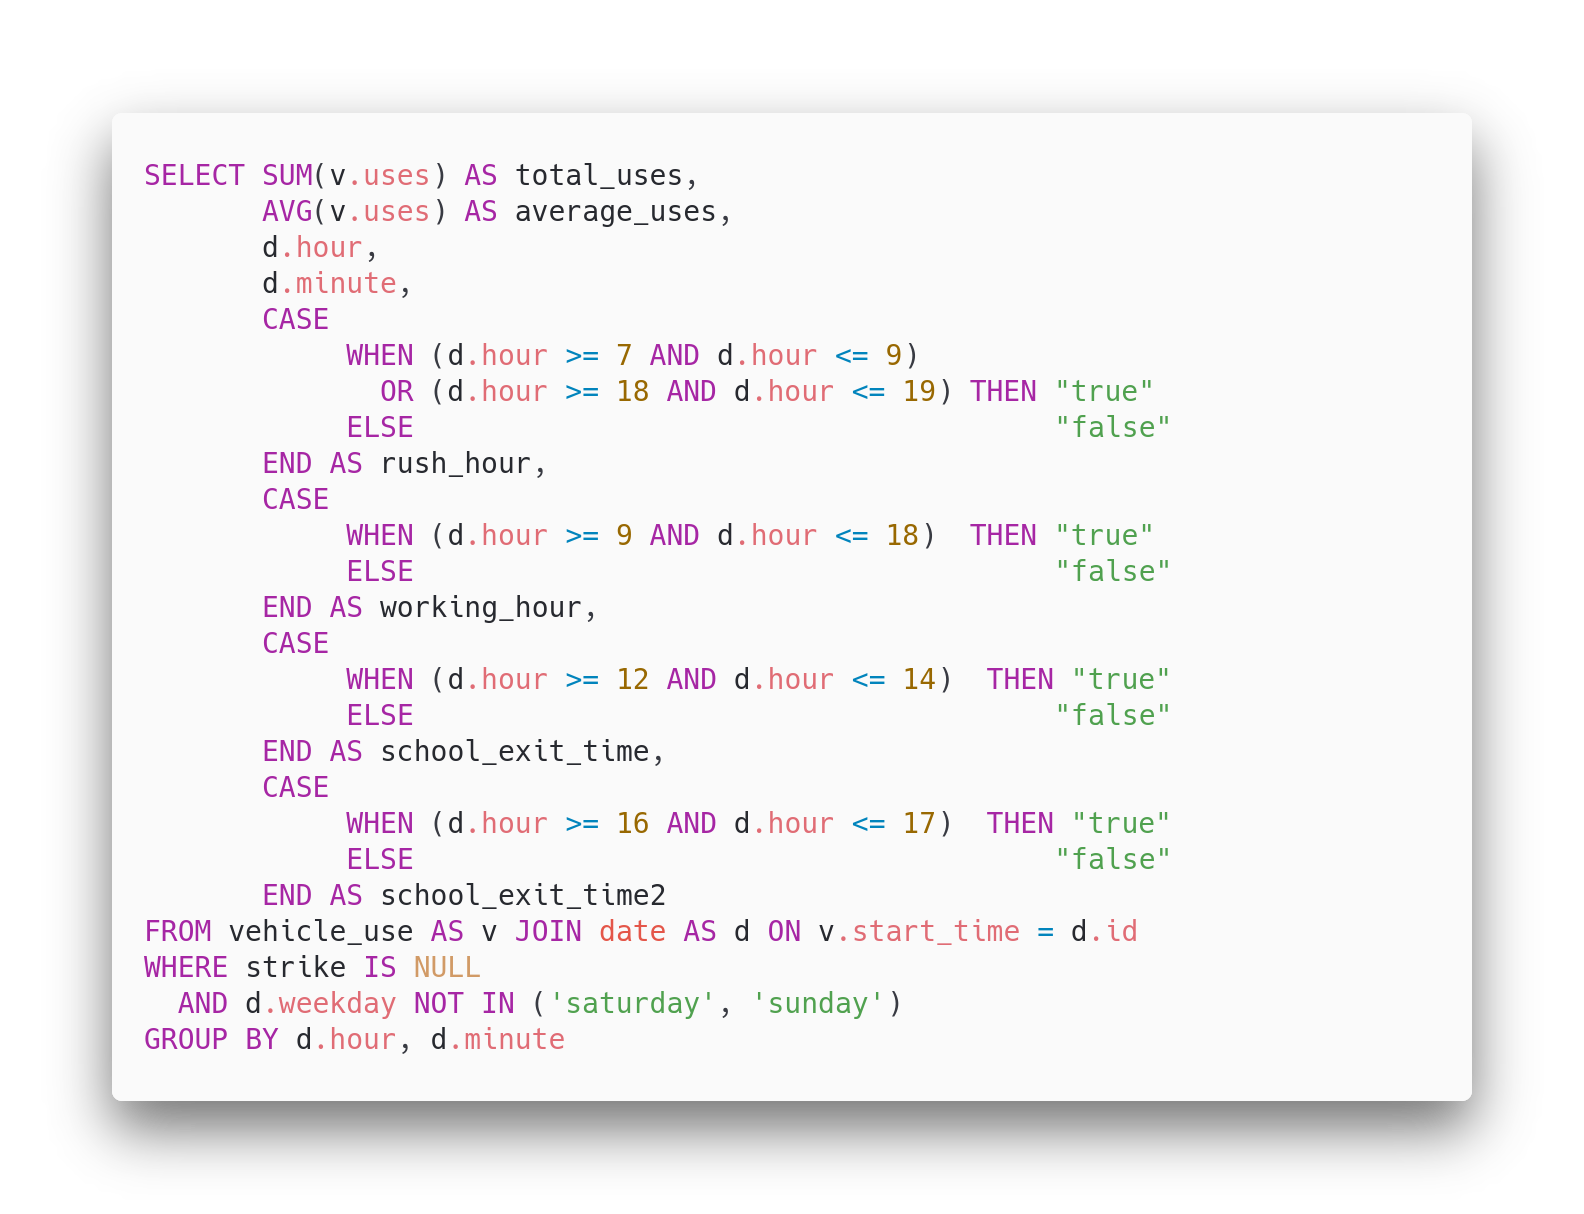
\includegraphics[width=\textwidth]{images/query6}                                                                                                                                   
\label{fig:query6}                                                                                                                                                           
\end{figure}
\iffalse
SELECT SUM(v.uses) AS total_uses,
	   AVG(v.uses) AS average_uses,
       d.hour,
       d.minute,
       CASE 
       		WHEN (d.hour >= 7 AND d.hour <= 9)   
           	  OR (d.hour >= 18 AND d.hour <= 19) THEN "true"
       		ELSE 								      "false"
       END AS rush_hour,
       CASE 
       		WHEN (d.hour >= 9 AND d.hour <= 18)  THEN "true"
       		ELSE 								      "false"
       END AS working_hour,
       CASE 
       		WHEN (d.hour >= 12 AND d.hour <= 14)  THEN "true"
       		ELSE 								      "false"
       END AS school_exit_time,
       CASE 
       		WHEN (d.hour >= 16 AND d.hour <= 17)  THEN "true"
       		ELSE 								      "false"
       END AS school_exit_time2
FROM vehicle_use AS v JOIN date AS d ON v.start_time = d.id
WHERE strike IS NULL
  AND d.weekday NOT IN ('saturday', 'sunday')
GROUP BY d.hour, d.minute
\fi



\begin{figure}[H]                                                                                                                                                            
\centering                                                                                                                                                                   
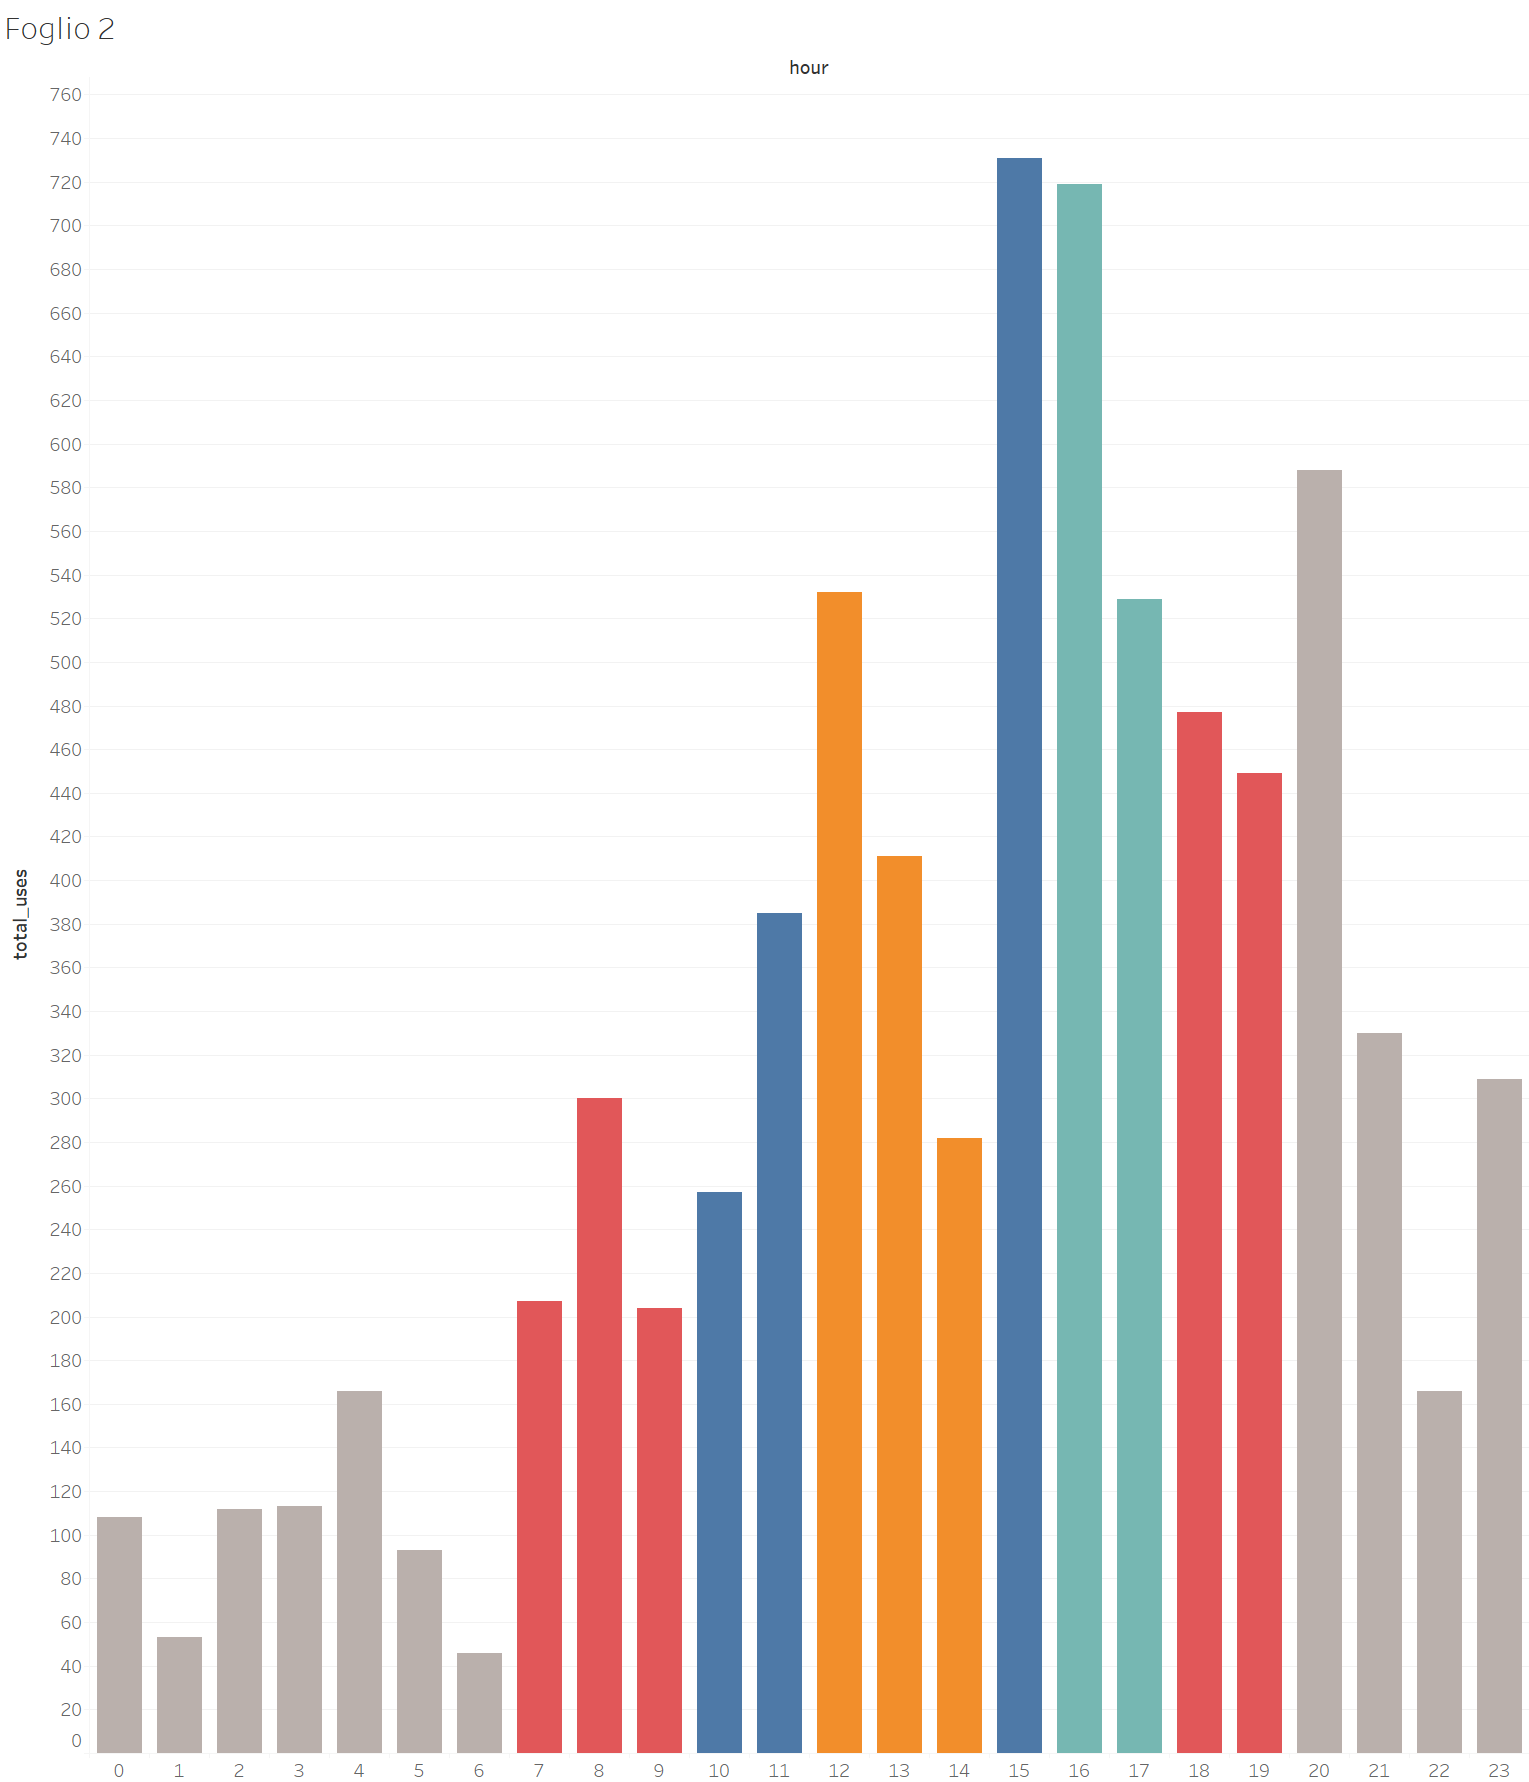
\includegraphics[width=\textwidth]{images/result6}                                                                                                                                   
\label{fig:result6}                                                                                                                                                           
\end{figure}